\section{Trær}
\begin{figure}[H]
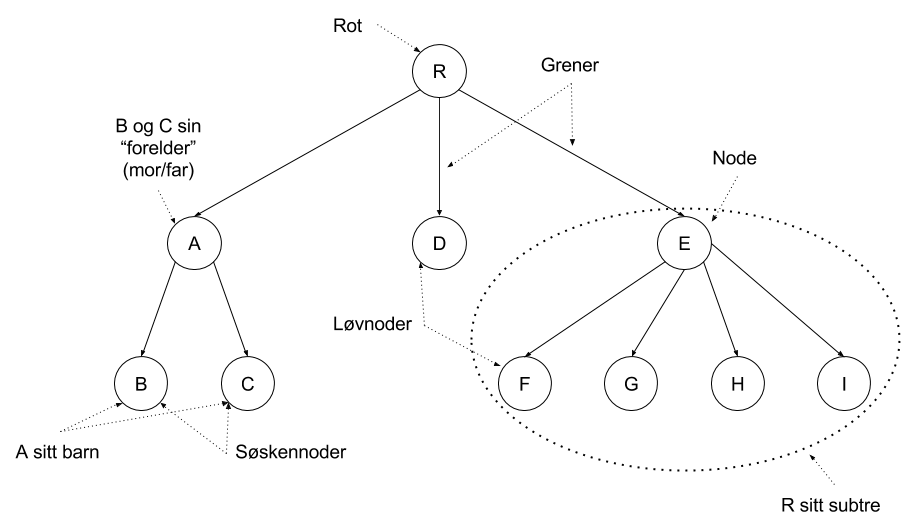
\includegraphics[scale=0.5]{images/traer}
\centering %centering the image
\caption{Tre}
\label{fig:trær}
\end{figure}

\begin{itemize}
    \item \textbf{Nivå for node} er antall grener som må passeres f.o.m. rot t.o.m. noden. Merk at rotnoden er på nivå 0.
    \item \textbf{Nodegrad} er antall barn (som er det samme som antall subtrær/undertrær) en node har.
    \item \textbf{Fritt tre} er at grenene ikke har retning, så alle nodene kan oppfattes som rotnode.
    \item \textbf{Rettet tre} vil si at grenene har retning, som i Figur \ref{fig:trær}.
    \item \textbf{Ordnet tre} vil si hvordan subtrærne/barna er ordnet i forhol til hverandre. Hvis det er viktig at A er til venstre, D i midten og E til høyre, er det et ordnet tre. Hvis rekkefølgen ikke har noe å si er det et uordnet tre.
    \item \textbf{Løvnode} er er node uten barn.
    \item \textbf{Indre node} er en node med barn.
    \item \textbf{Trehøyde} er maks antall grener som kan passeres f.o.m. rot t.o.m. løvnode.
    \item \textbf{$k$-grad-tre} vil si et tre der hver node kan ha maks $k$ barn. Posisjonen til barna er viktige.
    \item \textbf{Fullt $k$-grad-tre} er et $k$-grad-tre der alle indre noder har $k$ barn.
    \item \textbf{Komplett $k$-grad-tre} vil si et $k$-grad-tre der alle indre noder har $k$ barn, og enhver løvnode ligger på nivå $h$ eller $h - 1$, hvor $h$ er dybden (altså enten nederst i treet eller nest nederst). Antall noder på dybde $h$ er $k^h$. Trehøyden er $log_k n$ der $n$ er antall løvnoder.
\end{itemize}

\subsection{Implementasjon}
Hvordan vi implementerer en trestruktur avhenger av om vi har fast antall barn (f.eks. binære trær) eller variabelt antall barn (f.eks. B-trær).
\\\\
For hver av variantene har vi tatt med kjøretiden til to vanlige operasjoner:
\begin{itemize}
    \item finne forelder til en node
    \item finne barn nummer \textit{i} til en node
\end{itemize}

\noindent I generelle trær med fast antall barn har hver node er et objekt med en verdi, en peker til hver av barna og en peker til far.
\\\\
I generelle trær med variabelt antall barn er det to alternativer. Alternativ 1 er at hver node er et objekt med en verdi, en peker til sitt første barn (lengst til venstre), en peker til far og en til sin nærmeste bror til høyre for seg. I alternativ 2 utnytter vi at alle noder i et tre (untatt roten) har nøyatig én far. Vi lager en array. På plass nr \textit{i} står faren til node nummer \textit{i}, eller en peker til denne. Det blir da lett å finne faren, men for å finne barna til node \textit{i}, må vi søke gjennom arrayen etter tallet \textit{i}.

\begin{figure}[H]
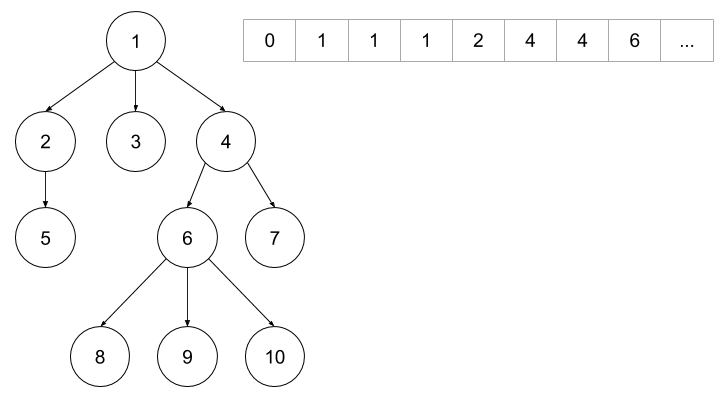
\includegraphics[scale=0.6]{images/fedrearray}
\centering %centering the image
\caption{Figuren viser et tre og den tilsvarende "fedrearrayen". Arrayen vil ha lke mange elementer som det er noder.}
\label{fig:fedrearray}
\end{figure}

\noindent Alternativ 3 er å lagre nodene i en array. HVert element i arrayen inneholder et objekt med verdien til noden og pekere til en lenket liste. Den lenkede listen inneholder pekere til barna.

\begin{figure}[H]
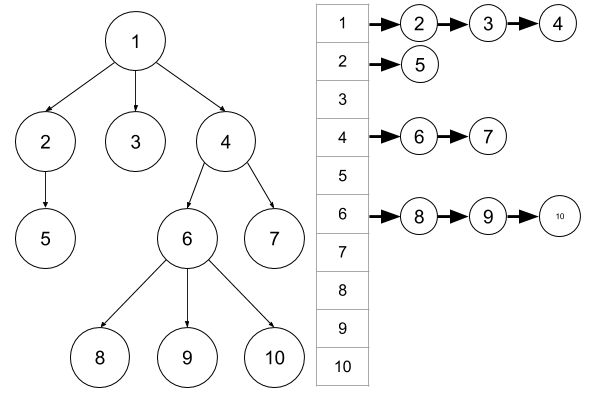
\includegraphics[scale=0.6]{images/alernativ3}
\centering %centering the image
\caption{Figuren viser alternativ 3.}
\label{fig:alternativ3}
\end{figure}

\subsection{Binære trær}
Binære trær er egentlig et 2-grad-tre, men dette navnet blir aldri brukt. Hver node har altså maks to barn og ordningen av høyre- og venstrebarn er viktig.

\begin{figure}[H]
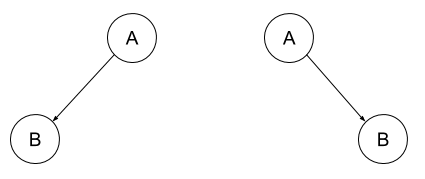
\includegraphics[scale=0.6]{images/binaeretraer}
\centering %centering the image
\caption{Disse to trærne er forskjellige!}
\label{fig:binaeretraer}
\end{figure}

\subsection{Minimale spenntrær}
\subsubsection{Kruskal}
\subsubsection{Prim}
Finner det minimale spenntreet i en graf. Altså den mengden med kanter som minimerer summen av vekter samtidig som grafen er sammenhengende. Det minimale spenntreet reflekterer ikke nødvendigvis de faktisk korteste veiene fra en node til en annen.
